\documentclass[]{elsarticle}
\usepackage{lmodern}
\usepackage{amssymb,amsmath}
\usepackage{ifxetex,ifluatex}
\usepackage{fixltx2e} % provides \textsubscript
\ifnum 0\ifxetex 1\fi\ifluatex 1\fi=0 % if pdftex
  \usepackage[T1]{fontenc}
  \usepackage[utf8]{inputenc}
\else % if luatex or xelatex
  \ifxetex
    \usepackage{mathspec}
    \usepackage{xltxtra,xunicode}
  \else
    \usepackage{fontspec}
  \fi
  \defaultfontfeatures{Mapping=tex-text,Scale=MatchLowercase}
  \newcommand{\euro}{€}
\fi
% use upquote if available, for straight quotes in verbatim environments
\IfFileExists{upquote.sty}{\usepackage{upquote}}{}
% use microtype if available
\IfFileExists{microtype.sty}{%
\usepackage{microtype}
\UseMicrotypeSet[protrusion]{basicmath} % disable protrusion for tt fonts
}{}
\ifxetex
  \usepackage[setpagesize=false, % page size defined by xetex
              unicode=false, % unicode breaks when used with xetex
              xetex]{hyperref}
\else
  \usepackage[unicode=true]{hyperref}
\fi
\hypersetup{breaklinks=true,
            bookmarks=true,
            pdfauthor={},
            pdftitle={Pragmatic language interpretation as probabilistic inference},
            colorlinks=true,
            citecolor=blue,
            urlcolor=blue,
            linkcolor=magenta,
            pdfborder={0 0 0}}
\urlstyle{same}  % don't use monospace font for urls
\usepackage{graphicx,grffile}
\makeatletter
\def\maxwidth{\ifdim\Gin@nat@width>\linewidth\linewidth\else\Gin@nat@width\fi}
\def\maxheight{\ifdim\Gin@nat@height>\textheight\textheight\else\Gin@nat@height\fi}
\makeatother
% Scale images if necessary, so that they will not overflow the page
% margins by default, and it is still possible to overwrite the defaults
% using explicit options in \includegraphics[width, height, ...]{}
\setkeys{Gin}{width=\maxwidth,height=\maxheight,keepaspectratio}
\setlength{\parindent}{0pt}
\setlength{\parskip}{6pt plus 2pt minus 1pt}
\setlength{\emergencystretch}{3em}  % prevent overfull lines
\providecommand{\tightlist}{%
  \setlength{\itemsep}{0pt}\setlength{\parskip}{0pt}}
\setcounter{secnumdepth}{0}

\title{\hyperdef{}{h.9p66emvfkv2}{\label{h.9p66emvfkv2}}{}Pragmatic language
interpretation as probabilistic inference}
\date{}

% Redefines (sub)paragraphs to behave more like sections
\ifx\paragraph\undefined\else
\let\oldparagraph\paragraph
\renewcommand{\paragraph}[1]{\oldparagraph{#1}\mbox{}}
\fi
\ifx\subparagraph\undefined\else
\let\oldsubparagraph\subparagraph
\renewcommand{\subparagraph}[1]{\oldsubparagraph{#1}\mbox{}}
\fi

 \newcommand{\denote}[1]{\mbox{ $[\![ #1 ]\!]$}}


\begin{document}
\maketitle

\begin{quote}
\emph{``... one of my avowed aims is to see talking as a special case or
variety of purposive, indeed rational, behavior ...''} -- Grice (1975,
p. 47)
\end{quote}

\subsection{Introduction}\label{introduction}

Language is central to the successes of our species; with language we
can coordinate our actions, learn from each other, and convey our
innermost thoughts. From sounds to syntax, natural languages provide
structured methods of combining discrete materials to generate an
infinite variety of sentences. Yet this discrete combinatorics does not
fully explain how speakers can use language so flexibly to achieve
social goals. The interpretation of a particular utterance in context
can itself be almost infinitely variable, depending on factors such as
the identity of the speaker, the physical context of its use, and the
previous discourse. While the systematization of structural features of
language is one of the proudest accomplishments of cognitive science
(e.g., Chomsky, 1965; Jackendoff, 2005; Goldberg, 2002), its contextual
flexibility -- its pragmatics -- has been stubbornly difficult to
formalize.

Grice (1975) presented an initial framework theory for pragmatic
reasoning, positing that speakers are taken to be cooperative, choosing
their utterances to convey particular meanings. Gricean listeners then
attempt to infer the speaker's intended communicative goal, working
backwards from the form of the utterance. This \emph{goal inference}
framework for communication has been immensely influential (e.g., Horn,
1984; Sperber \& Wilson, 1985; Clark, 1996; Levinson, 2000). But
attempts to build on these ideas by providing a specific set of formal
principles that allow the derivation of pragmatic inferences have met
with difficulty.

For example, the core of Grice's proposal was a set of
\emph{conversational maxims} (\textbf{see Glossary}; be truthful,
relevant, informative, and perspicuous) that could lead to
\emph{implicatures} -- inferences about speakers' intended meaning
--~when violated. Attempts to formalize the Gricean notion of
implicature have faltered (e.g., Hirschberg, 1985), and many
post-Gricean theories have instead proposed alternative sets of
principles (Sperber \& Wilson, 1985; Levinson, 2000). An important test
of the difficulty of this theoretical project is that the burgeoning
experimental psycholinguistic literature attempting to measure pragmatic
inference has found these principles only modestly useful (e.g., Breheny
et al., 2005; Huang \& Snedeker, 2009; Noveck \& Reboul, 2008). More
generally, informal theories of pragmatics make at best directional,
qualitative predictions with respect to data (which are often graded and
quantitative).

An alternative strand of Gricean thought has had more success in making
contact with data. Grice's core insight was that language use is a form
of rational action; thus, technical tools for reasoning about rational
action should elucidate linguistic phenomena. Such a goal-directed view
of language production has led to the development of engineering systems
for natural language generation (Reiter \& Dale, 1995) that have in turn
been applied as theories of human language production (e.g., Viethen \&
Dale, 2005). Concurrently, the tools of game-theory -- which allow for
the characterization of rational actions with respect to defined
utilities --~have provided a vocabulary for formal descriptions of
pragmatic phenomena (Benz et al., 2006). The recent work we focus on
here builds on these developments, combining them with a more detailed
view of cognition that arises from the Bayesian cognitive modeling
tradition.

Probabilistic, or Bayesian, models have been at the core of a set of
recent attempts to understanding the interplay between structured
representations and graded or statistical information (Tenenbaum et al.,
2011). These models have been an important tool for understanding
non-linguistic varieties of rational action, integrating belief
understanding with action planning (Baker, Saxe, \& Tenenbaum, 2009). A
critical feature of these models is that they use the probability
calculus to describe inferences under uncertainty. Within formal models
of pragmatics, this uncertainty stems from a variety of sources,
including uncertainty about speakers' goals and beliefs, uncertainty
about the discourse and broader context, and even uncertainty about the
meanings of words.

In the remainder of this paper we review the field of probabilistic
pragmatics. We begin by describing the \emph{``rational speech act''}
(RSA) model, and the growing body of empirical data supporting its
utility in explaining pragmatic reasoning. We next describe extensions
to RSA that allow it to be applied to non-literal uses of language like
hyperbole, irony and metaphor, to cases of vagueness and ambiguity, and
to complex interactions between pragmatics and compositional
syntax/semantics. We close with a discussion of broader applications of
-- and challenges for -- probabilistic pragmatics models.

\subsection{A ``rational speech act'' model
}\label{a-rational-speech-act-model}

The ``rational speech act'' (RSA) framework implements a social
cognition approach to utterance understanding. At its core, it captures
the idea (due to Grice, Lewis, and others) that speakers are assumed to
produce utterances to be helpful yet parsimonious, relative to some
particular topic or goal. Listeners then understand utterances by
inferring what such a helpful speaker must have meant, given what he
said. These two basic assumptions are formalized by viewing the speaker
as a utility-maximizing agent (where the effort of language production
is costly, but communicating information beneficial). The listener then
updates his beliefs via Bayesian inference.

The pragmatic listener infers the state of the world, \emph{w,} using
Bayes' rule, given the observation that the speaker chose a particular
utterance, \emph{u}:

$$P_L(w\textbar{}u) \propto P_S(u\textbar{}w)P(w)$$

The key assumption he must make is that the speaker is
\emph{approximately rational,} that is, that she has chosen her
utterances in proportion to the utility she expects to gain.

$$P_S(u\textbar{}w) \propto exp(\alpha
U(u;w))$$

The speaker chooses $u$ from a set of \emph{alternative utterances}
(see Outstanding Questions). The parameter $\alpha$
captures the extent to which the speaker maximizes her utility --
\emph{how} rational will she be. The basic speaker utility used in RSA
captures the social benefit of providing epistemic help to a listener:

$$U(u;w) = -\log P_Lit(w'\textbar{}u)$$

This expression measures how much information is provided to the
listener; in order to avoid an infinite recursion, the speaker is
assumed to consider a simpler listener, the \emph{literal listener}
$P_Lit$\emph{.} The literal listener again updates his beliefs in
accord with Bayesian inference, under the assumption that the literal
meaning of the utterance is true:

$$P_Lit(w\textbar{}u) \propto
\delta_{\denote{u}(w)}P(w)$$

This definition of the literal listener requires a semantic denotation
for each sentence, $\denote{u}$, in which a sentence
has the value true or false when applied to a particular state of
affairs (i.e. a truth-function on possible worlds). As we describe
briefly below, this denotation connects RSA to work in lexical and
compositional semantics (Dowty, Wall, \& Peters, 2012).\footnote{Though
  traditional Montagovian semantics uses binary truth values, it is also
  in principle possible in this model to use a semantics with
  real-valued truth functions, and perhaps even to construct a
  real-valued semantics from vector-based representations (e.g., Monroe
  \& Potts, 2015).}

Consider the scenario in Figure 1, in which speaker and listener share a
world of three faces -- one with hat and glasses (HG), one with glasses
only (G), and one with neither (N); one of these (known to the speaker
but not the listener) is the ``friend.'' The speaker says ``my friend
has glasses.'' Experimental participants tend to share the intuition
that this sentence refers to G and not HG or N (Stiller, Goodman, \&
Frank, 2015). Under RSA, listener L reasons about S (a simplified
internal representation of the speaker), who in turn reasons about Lit
(a yet more simplified internal model of the listener). Lit updates his
beliefs based on a straightforward denotation: ``glasses'' applies to
both G and HG, while ``hat'' applies only to HG. Thus
$P_Lit(w\textbar{}''hat'')$ places all probability on the friend
being HG, while $P_Lit(w\textbar{}''glasses'')$ is equal probability
on G and HG (see innermost thought bubbles in Figure 1). The speaker S
who intends to communicate that HG is the friend will thus tend to
choose the more informative ``hat'', but if she intends to communicate G
she will use ``glasses.'' Finally, upon hearing ``glasses'' the listener
L infers that this likely refers to G (via the counterfactual that if S
had been talking about HG, she would have said ``hat'' instead).

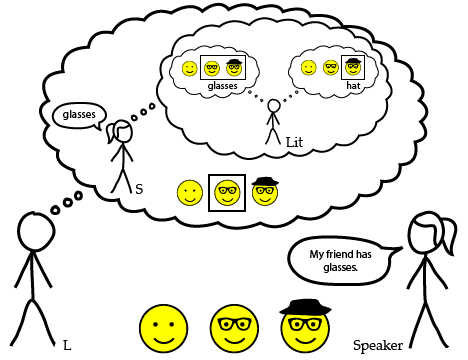
\includegraphics{images/media/image02.png}

\textbf{Figure 1}. Application of RSA-style reasoning to a signaling
game (bottom). Agents are depicted as reasoning recursively about one
another's beliefs.

In the simplest RSA model, as illustrated above, the speaker values
providing epistemic help --~information --~to the listener. But this can
be extended to create a more sophisticated speaker who is uncertain
about the world state, who avoids costly utterances, or who aims to
provide topic-relevant information (\textbf{see Box}). Connections to
other theoretical approaches and aspects of language then become
straightforward. For instance, by modifying the speaker utility, we can
model the notion of \emph{topic-relevant} information (see Box), which
connects to linguistic ideas about the ``question under discussion''
\cite{Roberts}. RSA can also be combined with the noisy
channel approach to language comprehension \cite{levy},
in order to explain the use of sentence fragments and prosodic stress to
communicate \cite{bergengoodman}. In sum, RSA models
replace Grice's variety of maxims with a single, utility-theoretic
version of the cooperative principle where the utilities can reflect a
complex, real-world agent.

\subsection{Empirical support for RSA }\label{empirical-support-for-rsa}

The example above (Figure 1) is an instance of a signaling game,
initially introduced by Lewis (1965). Such games are a valuable tool for
exploring pragmatic inferences in context, and experiments testing the
RSA framework have used games of this type to make quantitative
measurements of a variety of different inferences. For example, Frank \&
Goodman (2012) used a one-shot, web-based paradigm to present
participants with geometric shapes in a variety of different
configurations. Using a betting paradigm (participants were asked to
distribute \$100 between response options), these experiments collected
separate judgments about what a speaker would say, a listener would
interpret, and about baseline expectations for reference (corresponding
to the prior $P(w)$). The RSA model showed a tight, parameter-free fit
to listeners' aggregate judgements when a speaker model was combined
with empirical measurements of the prior distribution.

Although in this initial work RSA was used to simulate the behavior of
both speakers and listeners, most subsequent work has focused on the
behavior of listeners alone, assuming that RSA captures listeners'
(perhaps optimistic) assumptions about the rational behavior of
speakers. (Thus, RSA is `rational' in the sense of \emph{assuming} that
speakers are rational; a separate question is how rational speakers
actually \emph{are}; see production Box). Focusing on listeners, a
variety of other work has replicated and extended our initial finding
using similar signaling-game paradigms. In a tight replication of the
initial results, Qing \& Franke (2015) reproduced the basic findings and
explored a set of variants to the initial RSA utility function (see
Box). And Carstensen, Kon, \& Regier (2014) also found that RSA
predicted judgments in a communication game using much more complex
spatial language stimuli, albeit with somewhat noisier fits. Thus, RSA
with an epistemic utility can predict judgments in simple signaling
games across variations in both sample and stimulus.

One question raised by this initial work, is the level of recursion that
best fits human performance. The presentation of RSA given above is
stated in terms of a minimal recursion (a listener reasons about
speaker, who in turn reasons about a literal listener) but much greater
depths of reasoning are possible. Some evidence suggests that deeper
recursion is not common in participants' judgments, at least for basic
signaling games. Participants tend to show results close to chance-level
performance for signaling systems that require deeper levels of
recursion to find unique interpretations (Stiller, Goodman, \& Frank,
2011; Degen \& Franke, 2012; Vogel et al., 2013). More recently,
however, Degen \& Franke (2016) showed some evidence of deeper recursion
for a subpopulation of participants (\textasciitilde{}15\%) in a more
complex paradigm, consistent with some work on recursion in competitive
games (Camerer et al., 2002). This heterogeneity -- and its dependence
on individual and contextual differences --~is an interesting topic for
future work.

A number of other studies have tested RSA with utilities extended as
described in \textbf{Box}. For instance, a speaker might be expected to
produce a less informative utterance when the more informative one is
much harder to say. This tendency can be formalized by including a cost
term in the speaker's utility (see Box); with this modification, RSA
predicts the impact of production costs on interpretations of the
listener. Bergen et al. (2012), showed that participants in a reference
game are indeed sensitive to the cost, in dollars, of alternative
message choices. Degen \& Franke (CITE) tested the effect of production
difficulty by manipulating how quickly the speaker could type on an
on-screen keyboard; participants' inferences reflected this difficulty
as predicted. Additional work has included proxies for production cost
such as number of words and their frequencies (Nordmeyer et al., 2014;
Graf et al., 2016).

RSA provides a way to describe reasoning about classic linguistic
implicatures, in addition to ad-hoc signaling systems. Perhaps the
best-studied of these is the scalar implicature that ``some of the
letters had checks inside'' implicates that \emph{not all} did. Goodman
\& Stühlmuller (2013) measured participants' judgments about the
interpretations of quantifiers and number words in exactly this
situation and found that these judgments were well-predicted by RSA. In
addition, a critical feature of this study was the inclusion of an
epistemic manipulation (e.g., some of the letters had not been opened
yet). By using expected informativity to account for the speaker's
limited perceptual access (see Box), the model was able to predict
differing patterns of listener judgments based on different levels of
speaker uncertainty. These empirical findings are congruent with recent
explorations of the importance of epistemic reasoning in pragmatic
implicature (e.g., Bergen \& Grodner, 2012; Breheny et al., 2013). They
also highlight the way the RSA framework provides a (non-modular) theory
for interactions between language and non-linguistic cognition.

\subsection{Uncertainty about the speaker: Joint
reasoning}\label{uncertainty-about-the-speaker-joint-reasoning}

In the basic RSA model, the listener has a specific model in mind of how
a speaker will behave. But what should a listener do if he is not sure
which speaker model is appropriate? Recent work has answered this
question by positing a joint inference: Which kind of speaker am I
interacting with and what is the world like, given the utterance I
heard? Formally this \emph{uncertain} RSA (or uRSA) framework requires
only a small change:

$$P_L(w,s\textbar{}u) \propto
P_S(u\textbar{}w,s)P(s)P(w)$$

where $s$ parametrizes different speaker types. In practice, $s$ can
refer to any factor that might influence the speaker's behavior,
including a particular conversational topic, uncertainty about word
meanings, differing background knowledge, or general discourse context.
This modification allows uRSA to capture a much wider variety of
linguistic phenomena; intuitively, a uRSA listener is a more realistic
cognitive agent than the RSA listener, who was restricted to the
specifics of a very particular context and goal. To illustrate this
intuition, we provide three examples of phenomena captured by uRSA:
non-literal language, vagueness, and embedded implicatures.

Non-literal language -- utterances that are easily interpreted but not
``actually true'' -- is problematic for most formal models of language
understanding, including basic RSA. How can figurative tropes like
hyperbole, sarcasm, and metaphor be interpreted, and why are they used?
Under uRSA, these uses can be described as arising from uncertainty
about the topic of conversation. If the speaker is expected to provide
information relevant for a particular topic $t$ (see Box Utilities),
the pragmatic listener will only update his beliefs along this topical
dimension. The interaction between uncertainty about the speaker's
intended topic and her intended meaning about that topic can drive
complex interpretations.

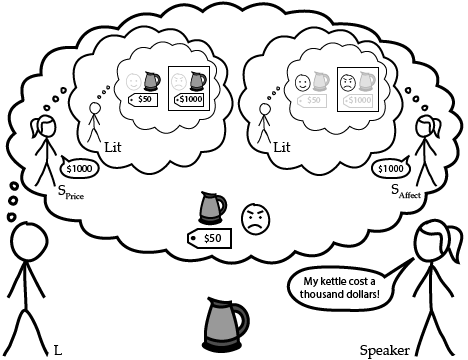
\includegraphics{images/media/image03.png}

\textbf{Figure 2}. Uncertain RSA-style reasoning applied to hyperbole.

Kao, et al (2014) investigated hyperbolic utterances such as ``the
electric kettle cost 1000\$'' In this example, the number \$1000 can
interpreted as conveying information about the speaker's affect, not the
actual price, in part because one thousand dollars is an implausibly
high price for a kettle. As shown in Figure 2, the uRSA model of Kao, et
al, captures this intuition by positing that the topic of the speaker's
utterance may be the actual price of the kettle, may be the speaker's
opinion about the price, or some combination of the two. The listener
does not know the topic, and so jointly infers it together with the
likely true price of the kettle and the speaker's affect. When the
uttered price is implausible this joint inference will yield a
non-standard topic and hence a non-literal interpretation. By extending
the space of affect to include both valence and arousal, Kao et al.
(2015) showed that the same model predicts verbal irony. In each case
the uRSA model accounts for almost all of the explainable variance in
human interpretations. A similar approach has been suggested for simple
metaphors (Kao, Bergen, Goodman, 2015), such as ``John is a shark,''
here the potential topics include not affect, but features of the
target, such as, how vicious John is and how likely he is to swim
underwater.

Another aspect of usage that could differ between speakers (and
contexts) is the effective meanings of words. For instance, scalar
adjectives like \emph{tall} and \emph{expensive} have an extremely
flexible meaning -- a \emph{tall man} is quite different in height than
a \emph{tall building}. In these cases, uRSA models can be used to infer
the precise meaning of words (Bergen, et al, 2016). In the case of
scalar adjectives, the uncertainty is over the threshold required: what
height is required before an object counts as tall? Critically, the
pragmatic listener infers this threshold, not the literal listener: the
pragmatic inference accounts for conflicting pressures for the threshold
to yield a meaning which is both true and informative; while a literal
inference would neglect informativity. The resulting uRSA model accounts
for three key phenomena of vague adjectives (Lassiter and Goodman,
2015): the inferred meaning depends on the class, there are borderline
cases, and the interpretations are subject to a \emph{sorites} paradox.
This approach to uncertainty about word meanings has been extended to
account for effects of ambiguity resolution (Scontras and Goodman, under
review), generic language (Tessler and Goodman, under review), habitual
statements (Tessler and Goodman, 2016), and manner implicatures (Bergen,
Levy, Goodman, 2016).

Finally, this uRSA approach allows for progress on an important puzzle
in recent discussions of pragmatic inference: embedded implicature
(Guerts \& Pouscoulous, 2009; Chemla \& Spector, 2011). Embedded
implicatures occur when quantifiers are nested within one another, as in

sentences like ``Exactly one letter is connected with some of its
circles.'' In these cases, some experimental evidence suggests that
participants access the interpretation that one letter is connected with
some \emph{but not all} of its circles, an interpretation that standard
Gricean theories cannot generate (Chemla \& Spector, 2011). Potts et al.
(2015) replicated these interpretations in a series of large-scale
experiments and confirmed that basic RSA models could not capture them.
An implementation of uRSA that operated over fully-compositional
semantic systems (Bergen, Levy, Goodman, 2016; Potts, et al, 2015)
showed a good fit to the overall pattern of data, however, supporting
the idea that uRSA is a useful framework for incorporating pragmatic
reasoning into more complex, compositional systems.

\subsection{Conclusions and future
directions}\label{conclusions-and-future-directions}

Context-dependence is one of the core features of natural language. Yet
because of the vagueness of theorizing about this context-dependence,
pragmatics has often been treated as a theoretical ``wastebasket'' into
which unexplained phenomena are thrown (Bar-Hillel, 1972). We have
argued that new formal theories of pragmatics make quantitative
predictions about a wide variety of phenomena that have previously been
considered too difficult to operationalize. These include implicature,
vagueness, non-literal language, and the myriad other cases where
linguistic meaning is changed by context. The key tool in this work is
the Rational Speech Act model, which builds upon and synthesizes a
number of formal traditions in the study of human inference, from game
theory to models of human reasoning. The RSA approach builds on existing
work on semantic representation -- using a compositional semantics
\emph{a la} Montague -- and contributes back to semantics by providing a
specific mechanism by which underspecified meanings become precise, in
context. Future work will need to engage with additional levels of
linguistic structure, such as discourse (Ascher, etc).

The RSA framework is a \emph{computational} level description of the
language user's competence, in Marr's (1983) parlance. There are many
possible ways a cognitive agent could implement RSA at the algorithmic
level. These alternatives must be evaluated for their ability to capture
the process of human language understanding and production (Degen \&
Tanenhaus, 2015; Nordmeyer \& Frank, 2014; see Box). Yet even in its
current form, RSA potentially suggests a new take on pragmatic language
processing phenomena -- one that is consistent with recent empirical
findings. In Gricean analyses, a violation of a maxim leads to reasoning
to ``repair'' the interpretation. Many theorists have inferred from this
idea of repair that pragmatic inferences should be slow (because they
depend on full semantic interpretation) and optional (because they only
happen after a violation). Both of these assumptions have been
challenged theoretically (e.g., Levinson, 2000) and empirically (e.g.,
Grodner et al., 2009). In contrast, RSA-style reasoning makes pragmatic
inferences a fundamental part of language comprehension, in which the
ultimate goal of all interpretation is to settle on the intended
meaning, given both the literal semantics of the utterance and the
broader pragmatic context. In this way, RSA is consistent with modern
psycholinguistic theories that emphasize interactive, incremental
processing (e.g., Degen \& Tanenhaus, 2015).

On the practical side, computing the predictions of RSA models can
become prohibitive when the number of world states or utterances grows
large. Further development of algorithms to implement RSA are needed,
with the goal of making predictions about a utterances in a broader
range of contexts. These extensions will likely include more complex
worlds; pragmatic alternatives with compositional structure; more
sophisticated, multi-part discourses; and utility structures that better
take into account the complexities of social interaction. These
developments may go together with new algorithms for learning aspects of
the underlying semantics, which will open up new applications for the
RSA approach in computational linguistics and artificial intelligence
(e.g., Goland, Liang, \& Klein, 2010; Vogel \& Potts, 2013; Munroe \&
Potts, 2015; Andreas \& Klein ??).

The work outlined in this review represents steps towards a
comprehensive, formal theory of language understanding in context. While
much further work will be required, RSA models and their extensions have
proven to be useful tools for explaining both qualitative and
quantitative empirical data across a wide range of tasks and contexts.
Language is central to the human experience. We hope our work sheds
light on how its structure and systematicity can still give rise to such
an astonishingly flexible communication system.

\subsection{DISPLAY ITEMS - 6 + Trends + Outstanding
Questions}\label{display-items---6-trends-outstanding-questions}

\subsubsection{Trends box}\label{trends-box}

\begin{itemize}
\item
  \begin{quote}
  Rational speech act (RSA) models provide a quantitative framework to
  capture intuitions about pragmatic reasoning in language
  understanding.
  \end{quote}
\item
  \begin{quote}
  Extensions to RSA that allow for joint reasoning about word meaning
  and speakers' goals can capture many otherwise puzzling phenomena
  including embedded implicatures, vagueness, hyperbole, irony, and
  metaphor.
  \end{quote}
\item
  \begin{quote}
  This framework can inform psycholinguistic processing experiments,
  linguistic theory, and scalable natural language processing models.
  \end{quote}
\end{itemize}

\subsubsection{Box: Outstanding questions
}\label{box-outstanding-questions}

\begin{itemize}
\item
  \begin{quote}
  \emph{Model details.} How deeply do human comprehenders recurse when
  reasoning about others intentions? Is depth of reasoning constant, or
  does it vary across situations? How are alternative utterances
  computed? Do they depend \emph{a priori} on the heard utterance of
  context?
  \end{quote}
\item
  \begin{quote}
  \emph{Learning}. How can pragmatic reasoning occur in situations where
  an agent has uncertainty about the meanings of words or how they are
  combined?
  \end{quote}
\item
  \begin{quote}
  How do ``Gricean'' utilities relate to non-linguistic social goals?
  How do cooperative and competitive goals mix in language use?
  \end{quote}
\item
  \begin{quote}
  \emph{Dialogue}. How do representations of utilities, possible goals,
  and the context more broadly evolve over the course of a conversation?
  \end{quote}
\item
  \begin{quote}
  \emph{Language change}. How and when does synchronic language use in
  pragmatic contexts lead to diachronic language change?
  \end{quote}
\item
  \begin{quote}
  \emph{Algorithmic challenges}. Given the potential complexity of
  recursive pragmatic computations, how is language processed so
  quickly? How can RSA models be ``scaled up'' for natural language
  processing tasks?
  \end{quote}
\item
  \begin{quote}
  \emph{Neural mechanisms.} What are the neural substrates of pragmatic
  language comprehension, and are they shared with other mentalistic
  reasoning?
  \end{quote}
\end{itemize}

\subsubsection{Box: Refinements to the speaker's
utility}\label{box-refinements-to-the-speakers-utility}

The (listener's belief about) the speaker's utility is central to the
RSA approach. The basic RSA model captures the speaker's need to be
\emph{informative} to a listener: $U(u; w) = \log
P_Lit(w\textbar{}u)$. Different utilities lead to different kinds of
speakers, which lead to different interpretations by the pragmatic
listener. Several utility refinements (and their combinations) have been
considered in recent work:

\begin{itemize}
\item
  \begin{quote}
  Utterance cost: In order to capture a tendency of speakers to be
  parsimonious we can simply add a cost term: $U(u; w) =
  \log P_Lit(w\textbar{}u) + cost(u)$. The cost may
  reflect actual production cost (such as number of words) or proxies
  such as word frequency. This extension yields effects similar to
  Grice's maxim of manner (cite).
  \end{quote}
\item
  \begin{quote}
  Speaker uncertainty: When the speaker does not have full knowledge of
  the world they should choose an utterance according to \emph{expected
  utility}: $U(u;k) = E_{P(w\textbar{}k)}{[}U(u;w){]}$, where $k$
  summarizes the speaker's knowledge or observations. This extension
  correctly predicts interactions between a speaker's knowledge and a
  listener's interpretations
  \cite{goodmanstuhllmueler}.
  \end{quote}
\item
  \begin{quote}
  Topic relevance: While it may be highly informative to convey detailed
  knowledge (such as the pattern of papers on my office desk), it is
  rarely \emph{relevant}. Relevance can be captured by introducing a
  topic of conversation (sometimes known as a Question Under Discussion,
  cite Roberts), and adjusting the epistemic utility to reflect only
  information about this topic: $U(u;w,t)=\log \sum_{w' st t(w')=t(w)} P_Lit(w'\textbar{}u)$.
  Because the topic may reflect previous interactions, this extension
  leads to a variety of discourse effects.
  \end{quote}
\item
  \begin{quote}
  Other social goals: Language is often used not just to inform, but
  also to flirt, insult, comfort, and to pursue myriad other social
  goals. Non-informational utilities, e.g. utility directed towards
  kindness, can produce behaviors that appear polite
  \cite{yoon}.
  \end{quote}
\end{itemize}

\subsubsection{Box: Children's developing pragmatic competence.
}\label{box-childrens-developing-pragmatic-competence.}

From a very early age, children are oriented towards communication
generally, understanding the function of language for information
transfer and repurposing their limited linguistic means to achieve a
wide variety of ends (Vouloumanos et al., 2012; Clark, 2014). In light
of this general early orientation, the literature on pragmatic
development specifically has been puzzling: older children very reliably
fail to make scalar implicatures under a range of circumstances (Noveck,
2001). In one striking example, five-year-olds endorsed the statement
that ``some of the horses jumped over the fence'' even when three out of
three of a set of horses had made the jump (Papafragou \& Musolino,
2003).

What explains this disconnect between early communicative successes and
later pragmatic failures? Early theorizing suggested that younger
children might not be able to make pragmatic computations generally
(Noveck, 2001), but this hypothesis appears unlikely given evidence that
younger children are sensitive to the pragmatic informativeness of
messages (Katsos \& Bishop, 2011;O'Neil \& Topolevic, 2001). More
recently, theorists have proposed that apparent difficulties with
pragmatic implicatures may have resulted from children's inadequate
knowledge of the specific lexical alternatives that compete in pragmatic
inferences (e.g., not understanding that ``some'' contrasts with
``all,'' leading to the implicature ``some but not all'') rather than
difficulty with pragmatic computations more generally (Barner, Brooks,
\& Bale, 2011).

Our work supports this ``alternatives hypothesis'' by providing evidence
for a range of implicature computations in young children. For example,
in a purely referential (or ``ad hoc'') task that did not use
quantifiers or other complex language, three-year-old children showed
signs of successful implicature computations (Stiller, Goodman, \&
Frank, 2015). And children in the same age range were able to use an
implicature to guess the meaning of a novel word (Frank \& Goodman,
2014). These findings support the idea that even young children are able
to make flexible pragmatic inferences in simple referential scenarios,
and are consistent with the application of RSA-style reasoning. Future
research will be required, however, to test whether RSA (or some
capacity-limited modification) could make quantitative predictions about
pragmatic development.

\subsubsection{Box: Producing referring expressions
}\label{box-producing-referring-expressions}

RSA stands for the ``rational speech act'' model, but does it imply that
speakers are truly rational? And if so, how can this conclusion be
integrated with the large body of evidence indicating that speakers are
egocentric, error prone, and subject to idiosyncratic production
preferences (Keysar et al., 2003; Lane, Groisman, \& Ferreira, 2008;
Gatt et al., 2013)?

Although our initial studies collected judgements about language
production in extremely restricted tasks (Frank \& Goodman, 2012), most
recent work using the RSA model has focused on modeling listeners'
judgements, rather than speakers' productions. One reason for this
choice is that often the most interesting pragmatic inferences come
about when speakers are not maximally informative. For example, in the
signaling game shown in Figure 1, helpful speakers will often
overspecify and say ``glasses and no hat'' (Bauman, Clark, \& Kaufman,
2014). But this seemingly non-pragmatic response may in fact be a
reasonable response to uncertainty about whether a conversational
partner will in fact draw the desired implicature.

More generally, speakers' production choices are a promising area for
future research using RSA models with a broader range of utility
functions (see Box). In the example above, the pragmatic speaker's
utility would take into account both the costs of production (adding
``and no hat'') and the likely costs of errors in comprehension by the
listener (the ``huh? which one?'' that might occur if the listener fails
to make the implicature -- or simply wants to be absolutely certain).
Intuitively, this tradeoff might lead to some of the observed patterns
of ``irrational'' behaviors: for example, if a speaker is less certain
of the denotation of a gradable adjective like ``big'' then she might be
more likely to use a color term as well (Gatt et al., 2013).

Nevertheless, it is clear that in their natural behavior, speakers make
production decisions under time pressure and a variety of cognitive
demands (CITE). Integrating these demands with the predictions of
utility-theoretic models should be an important challenge for future
work.

\subsubsection{Box: Language use and language
change}\label{box-language-use-and-language-change}

The pragmatic processes described by RSA models occur in the moment of
communication, but can have a set of effects that ripple out through
language as a whole. The construal of an individual communication event
can influence learning processes (see Box), which in turn can lead to
systematic changes in word meanings (Smith, Goodman, \& Frank, 2013).
Words that are too narrow in their denotation can be pragmatically
overextended (Kao, Bergen, \& Goodman, 2015), while words that are too
broad can be narrowed via implicature. Over time, word meanings may
converge to the appropriate level of ambiguity to enable efficient
communication (Piantadosi, Tily, \& Gibson, 2013).

These processes of change that promote efficient communication have been
explored extensively within the iterated learning paradigm. For example,
iterated transmission of an arbitrary communication system can lead to
the emergence of semantic regularities (Kirby, Cornish, \& Smith, 2008).
This framework can also be used to express the competing pressures of
learnability and communication. When languages are selected only to be
learnable, they often become degenerate, including only a single word
(Perfors \& Navarro, 2014). But when they include a countervailing
pragmatic pressure, expressive and compositional languages can emerge
(Kirby et al., 2015).

If pressures for efficient communication lead to language change, then
these pressures should be visible in the lexicons of human languages. A
recent body of evidence suggests that they are. Regier and colleagues
have argued that the typological distribution of languages in particular
semantic domains reflects the range of optimal communication systems
(e.g., Regier, Kay, \& Khetarpal, 2007; Kemp \& Regier, 2012; Xu \&
Regier, 2014). For example, although an infinity of possible ways of
expressing kinship relations are in principle possible, those that are
instantiated in natural languages tend to be a good balance between
expressivity and compression. And some recent evidence suggests that
communicative regularities may even be encoded at the level of the
entire lexicon (Lewis \& Frank, in press).

\subsubsection{Glossary}\label{glossary}

\begin{itemize}
\item
  \begin{quote}
  Rational speech act model (RSA). A class of probabilistic model that
  assumes that language comprehension in context arises via a process of
  recursive reasoning about what speakers would have said, given a set
  of communicative goals.
  \end{quote}
\item
  \begin{quote}
  Scalar implicature.
  \end{quote}
\item
  \begin{quote}
  Conversational maxims. A set of principles described by Grice (1975)
  \end{quote}
\end{itemize}

\end{document}
